\begin{figure*}[!t]
    \centering
    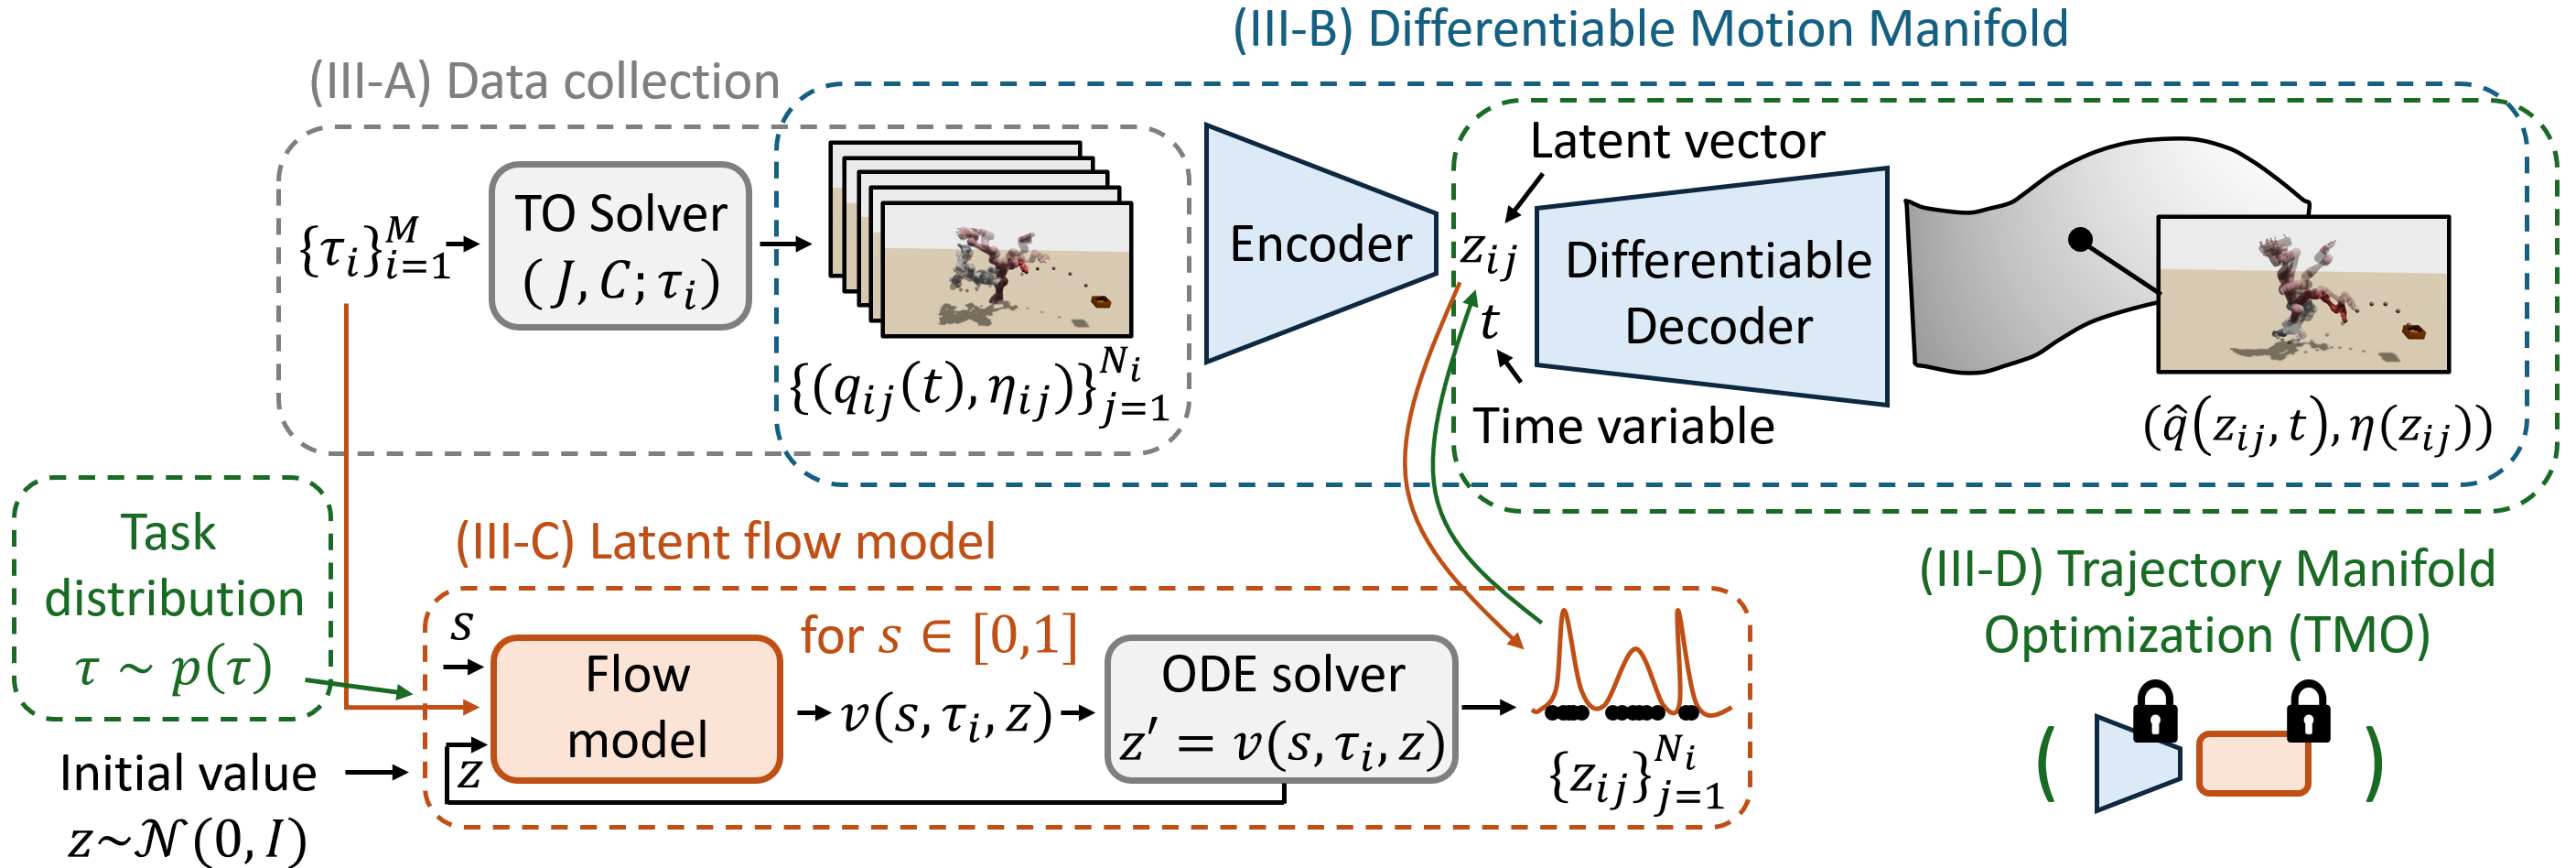
\includegraphics[width=0.8\textwidth]{method.PNG}
    \caption{Illustration of the overall training pipeline for the trajectory manifold. First, given a finite set of task parameters, we collect multiple, diverse trajectories for each task parameter using any existing Trajectory Optimization (TO) method. Second, we fit a Differentiable Motion Manifold (DMM) consisting of an encoder and a differentiable decoder -- by differentiable, we mean differentiable in time. Third, we learn a flow-based, task-conditioned distribution in the latent space. Lastly, we fine-tune the trajectory manifold by optimizing the decoder -- where we freeze the pre-trained encoder and latent flow model -- to ensure that the generated trajectories achieve the tasks and comply with kinodynamic constraints for all task parameters randomly sampled from the task distribution.}
    \label{fig:summary}
\end{figure*}

\section{Differentiable Motion Manifold Primitives}
\label{sec:method}


We begin with assumptions, notations, and problem definitions.  
Let the configuration be $q \in Q$ and the task parameter $\tau \in \mathcal{T}$ (e.g., the target box position for a throwing task).
For a fixed terminal time $T$, a smooth trajectory is denoted by $q(t)$ for $t \in [0,T]$, and an additional variable $\eta$ may be needed to fully specify a motion -- for example, in a throwing task, the release time $\eta \in (0,T)$ determines when the object is released at $q(\eta) \in Q$.  
The task-dependent objective function is $J(q(\cdot),\eta;\tau)$, and kinodynamic constraints such as self‑collisions, joint limits, and bounds on velocity, acceleration, jerk, and torque are expressed as $C(q,\dot q,\ddot q,\dddot q)\in\mathbb{R}^k \le 0$ with $C$ differentiable.  
We assume that, for each $\tau$, multiple globally or locally optimal motions $(q(t),\eta)$ exist.  
Our goal is to learn a model, given any $\tau \in \mathcal{T}$, generates multiple feasible motions $(q(t),\eta)$ that satisfy the constraints and optimize the objective.


Our framework consists of four steps. First, we collect multiple optimal trajectories by solving trajectory optimizations for each $\tau$ in section~\ref{sec:A}. Using these trajectories, we fit a differentiable motion manifold in section~\ref{sec:B}. 
In section~\ref{sec:C}, we train a task-conditioned motion distribution in the latent space. 
Lastly, in section~\ref{sec:D}, we fine-tune the motion manifold. The overall pipeline is visualized in Fig.~\ref{fig:summary}.

\subsection{Data Collection via Trajectory Optimizations}
\label{sec:A}
We collect multiple trajectories for each $\tau$ to enable subsequent manifold learning.  
Since sampling all $\tau \in \mathcal{T}$ is infeasible, we select a finite subset $\mathcal{T}_s=\{\tau_i\}_{i=1}^M$ that approximates $\mathcal{T}$.  
For each $\tau_i$, we solve
\begin{equation}
\min_{q(t),\eta} J(q(\cdot),\eta;\tau_i) \quad 
\text{s.t. } C(q,\dot q,\ddot q,\dddot q)\le0,\ \forall t\!\in[0,T].
\end{equation}
Specifically, we parameterize the trajectory as
\begin{equation}
\label{eq:parmetric_model}
q(t)=q_0+(q_T-q_0)(3-2s)s^2+s^2(s-1)^2\Phi(s)w,
\end{equation}
where $s=\tfrac{t}{T}$ and $q_0,q_T\in Q\subset\mathbb{R}^n$. 
The basis matrix is $\Phi(s)=[\phi_1(s), \ldots, \phi_{B}(s)] \in \mathbb{R}^{1\times B}$, where $\phi_i(s) = \exp(-B^2(s-\frac{i-1}{B-1})^2)$ and $B$ is the number of basis functions. The coefficient matrix $w\in\mathbb{R}^{B\times n}$. 
This parameterization satisfies the boundary conditions $q(0)=q_0$, $q(T)=q_T$, and $\dot q(0)=\dot q(T)=0$.  
We optimize over $(q_0,q_T,w)$ with diverse random seeds and initializations to collect diverse solutions $\{(q_{ij}(t),\eta_{ij})\}_{j=1}^{N_i}$.

\subsection{Learning Differentiable Motion Manifold}
\label{sec:B}
In this section, we propose a method to train a manifold of continuous-time, differentiable trajectories from the dataset $\{(q_{ij}(t),\eta_{ij})\}_{j=1}^{N_i}$.  
Following autoencoder-based manifold learning approaches~\cite{arvanitidis2017latent,lee2021neighborhood,yonghyeon2022regularized,lee2023explicit} and discrete-time MMPs~\cite{lee2023equivariant,lee2025motion}, we introduce an encoder $g$ and decoder $f$ with latent space $Z=\mathbb{R}^m$.  
The encoder maps a discretized trajectory $(q_1,\ldots,q_L)\in Q^L$ and $\eta$ to a latent variable $z\in Z$, i.e., $g((q_1,\ldots,q_L),\eta)=z$.  
Unlike discrete MMP decoders that take only $z$ and output a vectorized trajectory $(\hat{q}_1,\ldots,\hat{q}_L) \in Q^L$, our decoder takes $(z,t)$ and outputs $\hat q(z,t) \in Q$ and $\eta(z)$, with $\eta$ depending solely on $z$.  
Because $f(z,t)$ is differentiable in $t$, we refer to it as a \emph{differentiable decoder} (see Fig.~\ref{fig:dmm}).


\begin{figure}[!t]
    \centering
    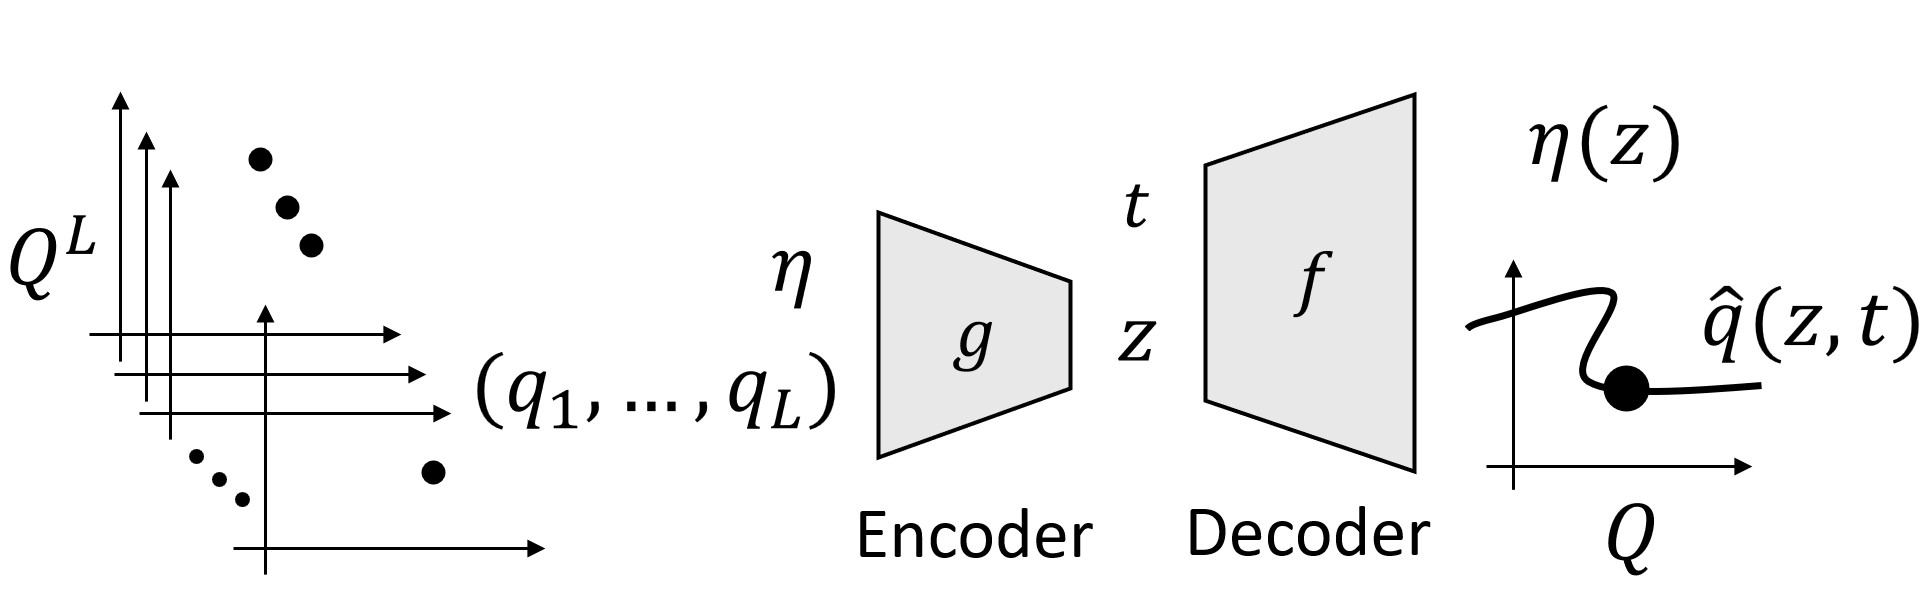
\includegraphics[width=0.9\linewidth]{DMM.jpg}
    \caption{The encoder takes $(q_1,\ldots,q_L) \in Q^L$ and $\eta$ and outputs the latent value $z$; the decoder maps $z$ and time variable $t$ to a configuration $\hat{q}(z,t) \in Q$ and $\eta(z)$.}
    \label{fig:dmm}
\end{figure}



The encoder and decoder are approximated with deep neural networks, denoted by $g_{\alpha}$ and $f_{\beta}=(\hat{q}_{\beta}, \eta_{\beta})$, respectively, with parameters $\alpha,\beta$, and trained to minimize the following loss function:
\begin{align}
    \label{eq:reconloss}
    {\cal L}_{{\rm recon}}(\alpha, \beta) := \frac{1}{M} \sum_{i} \frac{1}{N_i} \sum_{j} & \|\hat{q}_{\beta}(z_{ij}, t) - q_{ij}(t)\|_{c(t)}^2 \nonumber \\ & + \|\eta_\beta(z_{ij}) - \eta_{ij}\|^2, 
\end{align}
where $z_{ij} = g_{\alpha}((q_{ij}(t_1),\ldots, q_{ij}(t_L)), \eta_{ij})$, $t_l = \frac{l-1}{L-1}T$ for $l=1,\ldots, L$, and $\|\delta(t)\|_{c(t)}^2:=\int_{0}^T c(t) \delta^T(t) \delta(t) dt$ for some positive function $c(t)>0$.  
The positive function \( c(t) \) is introduced to fit more accurately on important parts along the time axis. For example, in the throwing task, the time around the throwing moment \( \eta \) should be given more weight.

Any neural network can be used for $f_\beta$.  
Inspired by deep operator learning~\cite{lu2019deeponet}, we adopt a linear basis function architecture for $\hat q_\beta$ that improves memory and computation efficiency:
\begin{equation}
\label{eq:lbfnn}
    \hat q_\beta(z,t) = \sum_{b=1}^{N_b} \psi_\beta^b(z)\,\theta_\beta^b(t),
\end{equation}
where $\psi_\beta^b: Z \to \mathbb{R}$ and $\theta_\beta^b:\mathbb{R}\to\mathbb{R}^n$ for $b=1,\ldots,N_b$ are neural networks.  
This structure avoids differentiating $\psi$ when computing time derivatives, reducing cost, and requires storing only $\psi(z)$ -- not the full network -- when inferring a trajectory for a fixed $z$, improving memory efficiency.

Given a sufficiently low-dimensional latent space $Z$ and the injective immersion conditions on $\hat{q}_{\beta}\colon z \mapsto \hat{q}_{\beta}(z, \cdot)$, we can interpret the set of trajectories $\{\hat{q}_{\beta}(z, \cdot) \mid z \in Z\}$ as an $m$-dimensional differentiable manifold of trajectories~\cite{arvanitidis2017latent,lee2023geometric,lee2022statistical,lee2024mmp++,yonghyeon2022regularized,heo2025isometric}.  
Although these conditions may not be strictly satisfied everywhere, they hold almost everywhere due to the smoothness properties of neural networks.  
Following established terminology~\cite{lee2023equivariant,lee2024mmp++,lee2025motion}, we adopt the term \emph{Differentiable Motion Manifold (DMM)} to denote this structure, as it captures the intrinsic low-dimensional manifold underlying the set of trajectories encoded by the model.





\subsection{Latent Flow Learning}
\label{sec:C}
This section describes how to fit a task‑conditioned density model $p(z|\tau)$ in the latent space of the learned differentiable motion manifold, adopting latent flow learning from MMFP~\cite{lee2025motion}.  
Let $z_{ij}$ be the latent encoding of $(q_{ij}(t),\eta_{ij})$ obtained from the trained encoder $g_{\alpha}$, giving a dataset of task–latent pairs $\big(\tau_i,\{z_{ij}\}_{j=1}^{N_i}\big)_{i=1}^M$.
Our goal is to train $p(z|\tau)$ so that, given a task $\tau$, we can sample $z$ and generate a motion via the decoder $f_\beta$, i.e., $z \mapsto f_\beta(z,\cdot)$.

Because $p(z|\tau)$ may be multimodal and highly nonconvex, we employ a flow‑based generative model~\cite{chen2018neural,lipman2022flow} for sufficient expressiveness.  
In latent space $Z$, we define a neural velocity field $v_\gamma(s,\tau,z)$ with parameters $\gamma$ and evolve it by
\begin{equation}
\label{eq:lsode}
    \frac{dz}{ds} = v_\gamma(s,\tau,z), \quad s \in [0,1],
\end{equation}
treating $p_\gamma(z|\tau)$ as the pushforward of a Gaussian prior $p_0(z)$.  
Sampling from $p_\gamma(z|\tau)$ involves drawing $z_0\sim p_0$ and integrating the ODE from $s=0$ to $s=1$.  
We train $v_\gamma$ using flow matching~\cite{lipman2022flow}, a simulation‑free method that is more efficient than maximum‑likelihood training.

Finally, by sampling $z \sim p_\gamma(z|\tau)$ and decoding with $f_\beta$, we generate motions for any given $\tau$.  
We refer to this framework as \emph{Differentiable Motion Manifold Flow Primitives (DMMFP)}.


\subsection{Trajectory Manifold Optimization}
\label{sec:D}
Trajectories generated by DMMFP are not guaranteed to satisfy kinodynamic constraints.  
Moreover, since the dataset covers only a finite set of task parameters \( \{\tau_i\}_{i=1}^M \), performance on unseen \( \tau \in \mathcal{T} \) is not guaranteed.  
To address this, we propose \emph{Trajectory Manifold Optimization (TMO)} to fine‑tune the manifold so that generated trajectories both achieve the task for all $\tau \in \mathcal{T}$ and satisfy the constraints.

Let $g_\alpha$, $f_\beta$, and $p_\gamma$ be the pre‑trained encoder, decoder, and latent flow.  
We fine‑tune only the decoder parameters $\beta$, keeping $\alpha$ and $\gamma$ fixed.  
Jointly tuning all parameters would require backpropagation through the sampled latent values and the ODE solver, making training computationally prohibitive, whereas adjusting $\beta$ alone is both efficient and sufficient to modify the manifold.

Define $U(S)$ as the uniform distribution over a set $S$.  
We introduce the task loss
\begin{align}
\label{eq:taskloss}
    {\cal L}_{\rm task}(\beta) := \mathbb{E}_{t, \tau, z}\Big[ &J(\hat{q}_\beta(z, \cdot), \eta_\beta(z); \tau) \nonumber \\ &+ W^T \big({\rm ReLU} (C(t, z, \beta))^2\big) \Big],
\end{align}
where $t \sim U([0,T])$, $\tau \sim U(\mathcal{T})$, and $z \sim p_\gamma(z|\tau)$.  
Here,
\begin{equation}
C(t,z,\beta) = C\!\big(\hat q_\beta, \tfrac{\partial}{\partial t}\hat q_\beta, \tfrac{\partial^2}{\partial t^2}\hat q_\beta, \tfrac{\partial^3}{\partial t^3}\hat q_\beta\big) \in \mathbb{R}^k,
\end{equation}
and $W \in \mathbb{R}^k$ is a positive weight vector.  
The first term in \eqref{eq:taskloss} enforces task success, while the second penalizes constraint violations.  
Sampling $\tau \sim U(\mathcal{T})$ improves generalization, as the model is no longer limited to the subset $\mathcal{T}_s$ previously used for training.


Finally, adding the reconstruction loss \eqref{eq:reconloss} with fixed $\alpha$, we minimize
\begin{equation}
{\cal L}(\beta) = w_{\rm recon}{\cal L}_{\rm recon}(\beta) + {\cal L}_{\rm task}(\beta),
\end{equation}
where $w_{\rm recon}>0$.  
We refer to this fine‑tuning process as \emph{Trajectory Manifold Optimization (TMO)}.
